\input ../SlidePreamble
\input ../preamble


\begin{document}

{\Huge

  \centerline{\bf TTIC 31230, Fundamentals of Deep Learning}
  \bigskip
  \centerline{David McAllester, Autumn 2023}
  \vfill
  \vfil
  \centerline{The Mathematics of Diffusion Models}
  \vfill
  \centerline{McAllester, arXiv January 2023}
    \vfill
  \vfill

\slidetwo{Denoising Diffusion Probabilistic Models (DDPM)}{Ho, Jain and Abbeel, June 2020}

\centerline{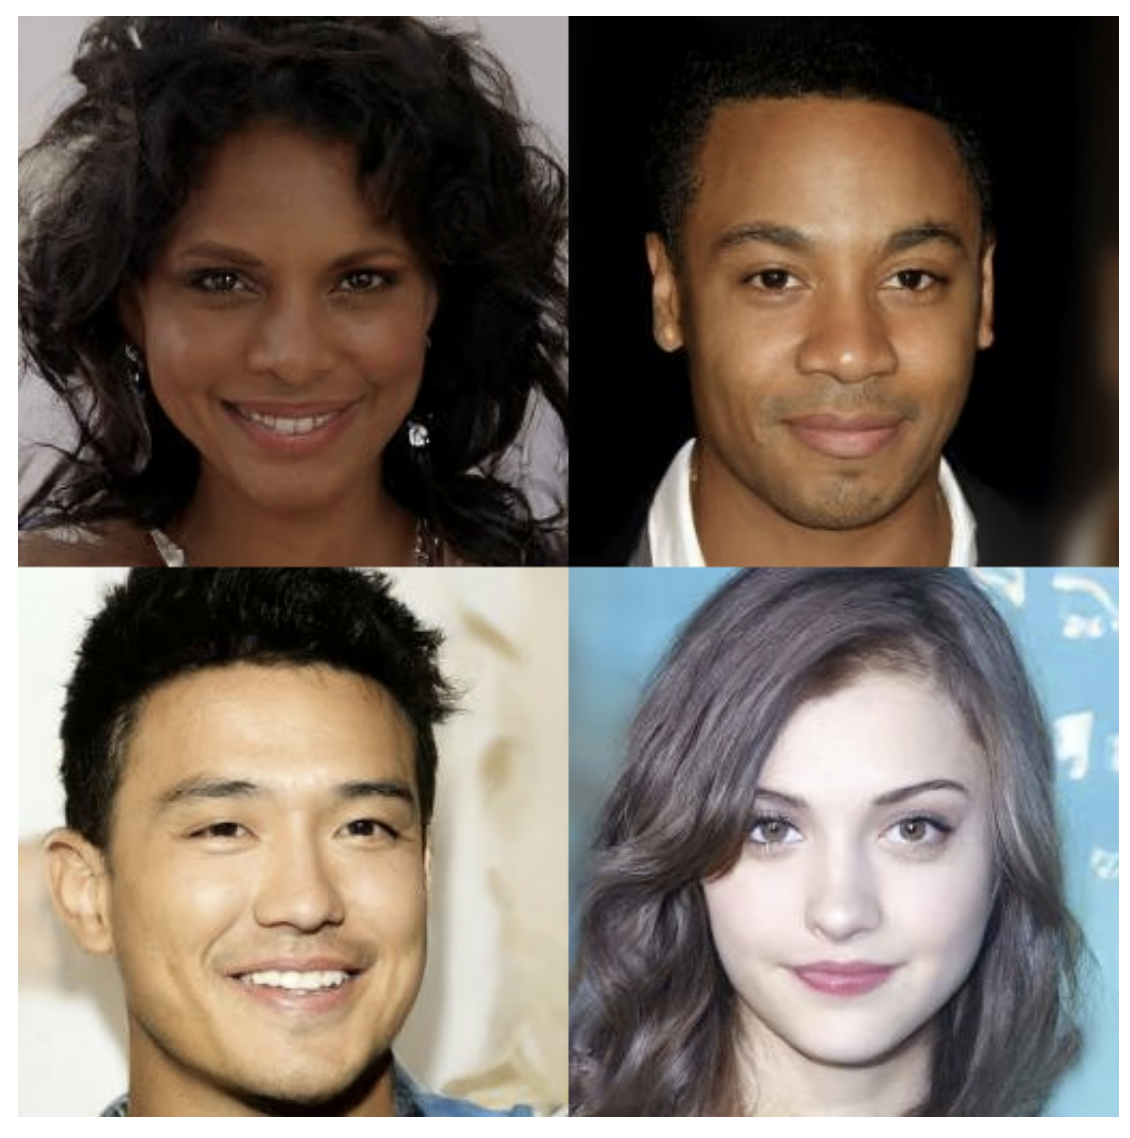
\includegraphics[width = 4in]{\images/DiffCeleb}}


\slide{Markovian VAEs}

A diffusion models computes and inverts a sequence

\vfill
\centerline{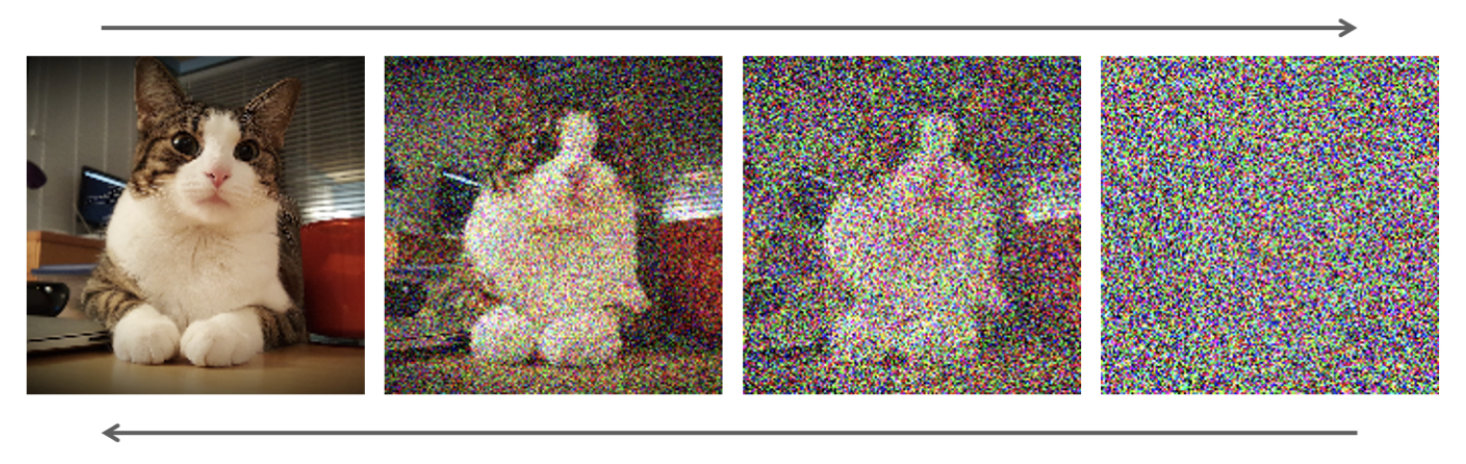
\includegraphics[width = 7in]{\images/DiffSequence}}

\vfill
So does an autoregressive language model

\vfill
{\huge
\centerline{{\color{red} [Sally talked to John]} $\stackrel{\rightarrow}{\leftarrow}$ {\color{red} [Sally talked to]}
$\stackrel{\rightarrow}{\leftarrow}$ {\color{red}[Sally talked]} $\stackrel{\rightarrow}{\leftarrow}$ {\color{red}[Sally]}}
}


\slide{Markovian VAEs}


\centerline{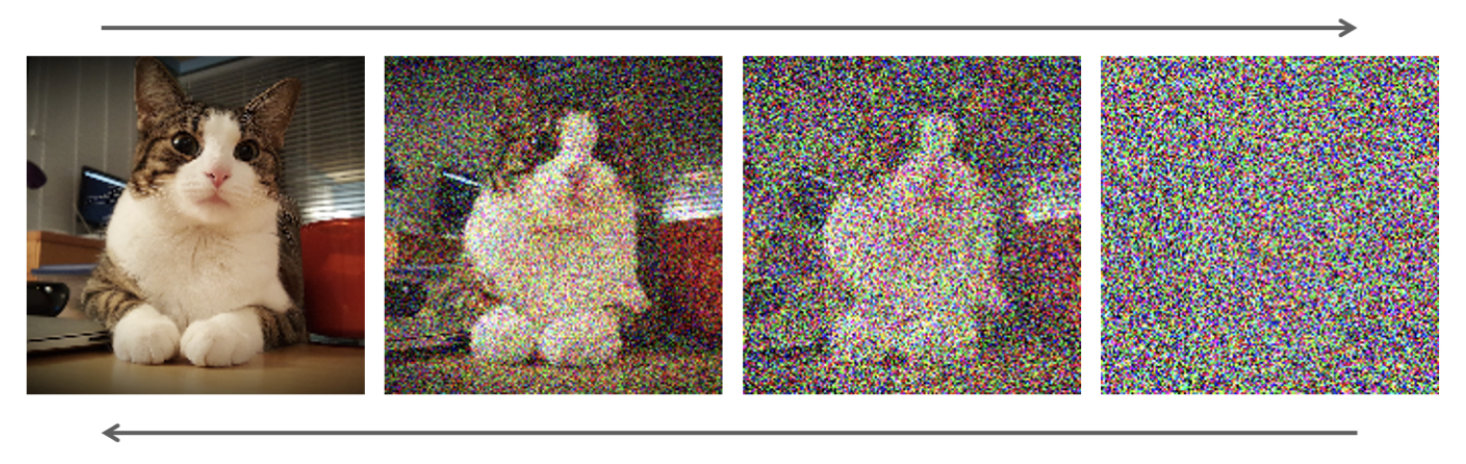
\includegraphics[width = 7in]{\images/DiffSequence}}

\vfill
{\huge
\centerline{{\color{red} [Sally talked to John]} $\stackrel{\rightarrow}{\leftarrow}$ {\color{red} [Sally talked to]}
$\stackrel{\rightarrow}{\leftarrow}$ {\color{red}[Sally talked]} $\stackrel{\rightarrow}{\leftarrow}$ {\color{red}[Sally]}}
}

\vfill
\centerline{$y \stackrel{\rightarrow}{\leftarrow} z_1  \stackrel{\rightarrow}{\leftarrow} \cdots \stackrel{\rightarrow}{\leftarrow} z_N$}

\slide{Markovian VAEs}
\centerline{$y \stackrel{\rightarrow}{\leftarrow} z_1  \stackrel{\rightarrow}{\leftarrow} \cdots \stackrel{\rightarrow}{\leftarrow} z_N$}

\vfill
{\bf Encoder}: $\pop(y)$, $P_\enc(z_1|y)$, and $P_\enc(z_{\ell+1}|z_\ell)$.


\vfill
{\bf Generator}: $P_\pri(z_N)$, $P_\gen(z_{\ell-1}|z_\ell)$, $P_\gen(y|z_1)$.

\vfill
The encoder and the decoder define distributions $P_\enc(y,\ldots,z_N)$ and $P_\gen(y,\ldots,z_N)$ respectively.

\slide{The Markovian ELBO}

{\Large
\begin{eqnarray*}
H(y) & = & E_\enc\left[- \ln\frac{P_\enc(y)P_\enc(z_1,\ldots,z_N|y)}{P_\enc(z_1,\ldots,z_N|y)}\right]\\
  \\
  \\
  & = & E_\enc\left[ - \ln\frac{P_{\color{red} \enc}(y|z_1)P_{\color{red} \enc}(z_1|z_2)\cdots P_{\color{red} \enc}(z_{N-1}|z_N)P_{\color{red} \enc}(z_N)}
  {P_\enc(z_1|z_2,y)\cdots P_\enc(z_{N-1}|z_N,y)P_\enc(z_N|y)}\right] \\
   \\
   \\
  & {\color{red} \leq} & E_\enc\left[ - \ln\frac{P_{\color{red} \gen}(y|z_1)P_{\color{red} \gen}(z_1|z_2)\cdots P_{\color{red} \gen}(z_{N-1}|z_N)P_{\color{red} \gen}(z_N)}
  {P_\enc(z_1|z_2,y)\cdots P_\enc(z_{N-1}|z_N,y)P_\enc(z_N|y)}\right] \\
\\
\\
 & = & \left\{\begin{array}{l}E_\enc\;[-\ln P_\gen(y|z_1)]
                             \\ \\ + \sum_{i=2}^N  \; E_\enc\; KL(P_\enc(z_{i-1}|z_i,y),\;P_\gen(z_{i-1}|z_i)) \\
                             \\ + E_\enc\; KL(P_\enc(Z_N|y),p_\gen(Z_N))\end{array}\right.
\end{eqnarray*}
}

\slide{Markovian VAEs}

\centerline{$y \stackrel{\rightarrow}{\leftarrow} z_1  \stackrel{\rightarrow}{\leftarrow} \cdots \stackrel{\rightarrow}{\leftarrow} z_N$}

\vfill
\begin{itemize}
\item autoregressive models

\vfill
\item diffusion models

\vfill
\item StyleGan? (layers of resolution)

\vfill
\item U-Nets? (layers of resolution)
\end{itemize}

\vfill
A grand unified theory (GUT) of generative AI?

\slide{Diffusion Models}
\centerline{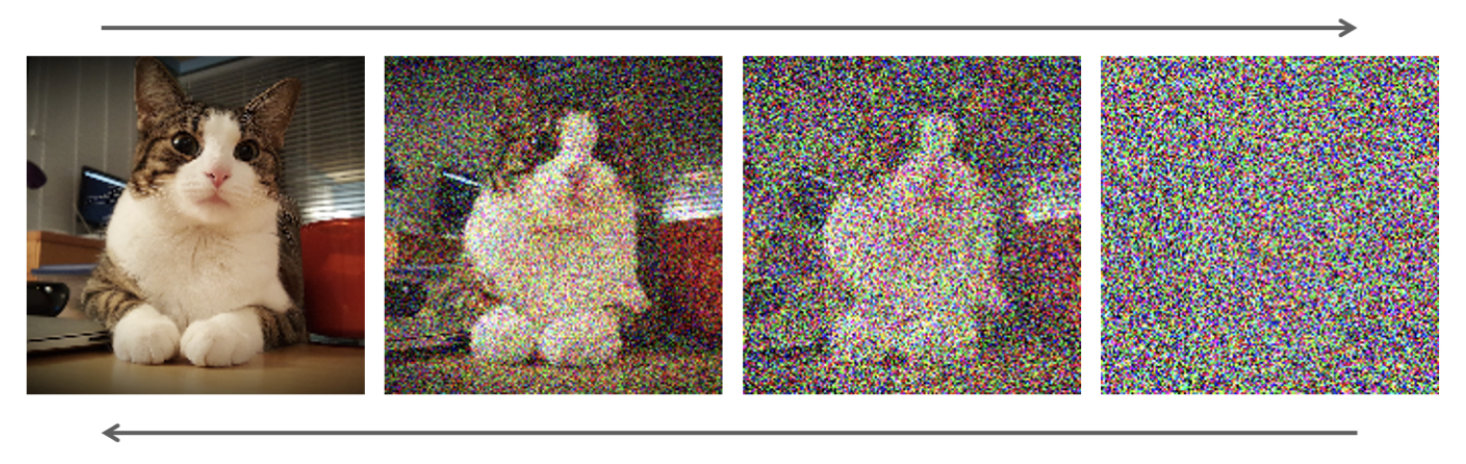
\includegraphics[width = 2in]{\images/DiffSequence}}

Consider a discrete time process $z(0),z(\Delta t),z(2\Delta t),z(3\Delta t),\ldots$
{\huge
\begin{eqnarray*}
  z(0) & = & y,\;\;\;y \sim \pop(y) \\
  \\
  z(t+\Delta t) & = & z(t) + \epsilon\sqrt{\Delta t},\;\;\;\epsilon \sim {\cal N}(0,I)
\end{eqnarray*}
}
A sum of two Gaussians is a Gaussian whose {\bf variance} is the sum of the two variances.

\vfill
$$z(t+n\Delta t) = z(t) + \sqrt{n\Delta t}\; \epsilon,\;\;\;\epsilon \sim {\cal N}(0,I)$$

\vfill
Here $\sqrt{n \Delta t}$ is the {\bf standard deviation} of the added noise.

\slide{SDE Notation}
In these slides $\epsilon$ will be a random variable drawn from ${\cal N}(0,I)$.

\vfill
This correspods to ``$dB$'' in standard notation for SDEs.

\vfill
{\huge
\begin{eqnarray*}
  z(t+\Delta t) & = & z(t) + \mu(z,t)\Delta t + \sigma(z,t)\epsilon\sqrt{\Delta t} \\
  \\
  dz & = & \mu(z,t)dt + \sigma(z,t)dB
\end{eqnarray*}
}

\vfill
The first expression is longer but seems clearer to me.

\vfill
The SDE denotes the limit as $\Delta t$ in the first equation goes to zero.

\slide{The Diffusion SDE}

\vfill
For the diffusion process (Brownian motion) we have

\vfill
{\huge
\begin{eqnarray}
  z(0) & = & y,\;\;\;y \sim \pop(y) \nonumber \\
  \nonumber \\
  z(t+\Delta t) & = & z(t) + \epsilon\sqrt{\Delta t} \label{forward} \\
  \nonumber \\
  dz & = & dB \nonumber
\end{eqnarray}
}

\vfill
For diffusion we get that (\ref{forward}) holds for all $t$ and $\Delta t$.

\slide{Probability Notation}

In these slides unsubscripted probability notation, such as

\vfill
$$P(z(t+\Delta t)|z(t)),$$

\vfill
or a conditional expectation such as

\vfill
$$E[f(y)|z(t)] = E_{y \sim P(y|z_t)}[f(y)],$$

\vfill
refer the joint distribution on $y$ and $z(t)$ defined by diffusion.

\slide{Markovian ELBO}

For any Markovian VAE we have

\vfill
{\Large
\begin{eqnarray}
  - \ln \pop(y) & = & - \ln\frac{P(z_N)P(z_{N-1}|z_N)\cdots P(z_1|z_2)P(y|z_1)}{P(z_N|y)P(z_{N-1}|z_N,y)\cdots P(z_1|z_2,y)} \nonumber\\
  \nonumber \\
  \nonumber \\
  H(y) & = & \left\{\begin{array}{l} E[KL(P(z_N|y),\;P(z_N))] \\ \\ + \sum_{i=2}^N  \; E[KL(P(z_{i-1}|z_i,y),\;P(z_{i-1}|z_i))] \\ \\ +\;E[\ln -P(y|z_1)] \end{array}\right. \label{Markov-eq} \\
  \nonumber\\
  \nonumber\\
  & \leq & \left\{\begin{array}{l} E[KL(P(z_N|y),\;P_{\color{red} \gen}(z_N))] \\ \\ + \sum_{i=2}^N  \; E[KL(P(z_{i-1}|z_i,y),\;P_{\color{red} \gen}(z_{i-1}|z_i))] \\ \\ E[- \ln P_{\color{red} \gen}(y|z_1)] \end{array}\right. \;\;\;~\label{Markov-ELBO}
\end{eqnarray}
}

\slide{Reverse-Time Probabilities}

In the limit of small $\Delta t$ it is possible to derive the following.

\begin{eqnarray*}
  P(z(t - \Delta t)|z(t),y) & = & {\cal N}\left(\begin{array}{l}z(t) + \frac{\Delta t(y - z(t))}{t},\;\; \Delta t I\end{array}\right) \\
  \\
  \\
  P(z(t - \Delta t)|z(t)) & = & {\cal N}\left(\begin{array}{l} z(t) + \frac{\Delta t(E[y|t,z(t)] - z(t))}{t}, \;\; \Delta t I\end{array}\right)
\end{eqnarray*}


\slide{The Reverse-Diffusion SDE}

$$P(z(t - \Delta t)|z(t)) = {\cal N}\left(\begin{array}{l} z(t) + \frac{\Delta t(E[y|t,z(t)] - z(t))}{t}, \Delta t I\end{array}\right)$$

\vfill
This equation defines a reverse-diffusion SDE which we can write as

{\huge
$$z(t - \Delta t) = z(t) + \left(\frac{E[y|t,z(t)] - z(t)}{t}\right)\Delta t +  \epsilon\sqrt{\Delta t}$$
}

\slide{Understanding Reverse Diffusion}

{\huge
$$z(t - \Delta t) = z(t) + \left(\frac{{\color{red} E[y|t,z(t)]} - z(t)}{t}\right)\Delta t +  \epsilon\sqrt{\Delta t}$$
}

\vfill
\centerline{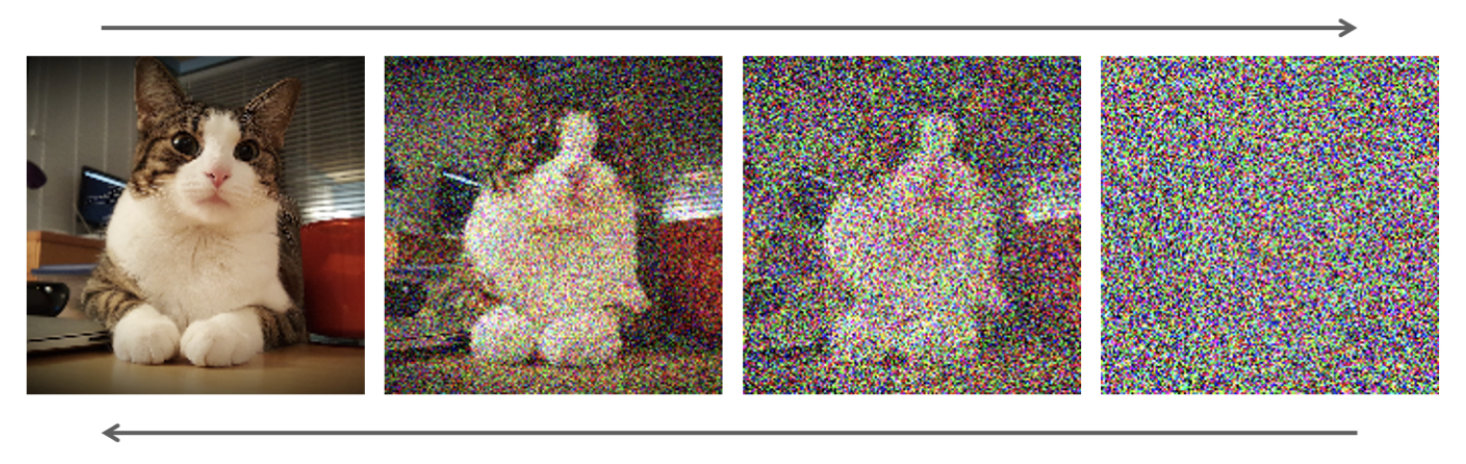
\includegraphics[width = 7in]{\images/DiffSequence}}

\vfill
$E[y|t,z]$ is averaging over many possible source images $y$.

\slide{Estimating $E[y|t,z(t)]$}

$$z(t - \Delta t) = z(t) + \left(\frac{E[y|t,z(t)] - z(t)}{t}\right)\Delta t +  \epsilon\sqrt{\Delta t}$$

\vfill
We can train a denoising network $\hat{y}(t,z)$ to estimate $E[y|t,z(t)]$ using
$$\hat{y}^*(t,z) = \argmin_{\hat{y}} \;E \;(\hat{y}(t,z(t)) - y)^2$$


\vfill
Assuming universality $\hat{y}^*(t,z) = E[y|t,z]$.

\slide{Estimating $E[y|t,z(t)]$}

\vfill
If the population values are scaled so as to have scale 1, then the scale of $z(t)$ is $\sqrt{1+t}$.

\vfill
$$\hat{y}^* = \argmin_{\hat{y}} E_{t,z(t)} \; (\hat{y}(t,z/\sqrt{1+t}) - y)^2$$

\vfill
\begin{eqnarray*}
\hat{E}[y|t,z(t)] & = & \hat{y}^*(t,z/\sqrt{1+t})) \\
\end{eqnarray*}

\slide{KL-Divergence}

{\huge
\begin{eqnarray*}
  H(y) & = & \left\{\begin{array}{l} E[KL(P(z_N|y),\;P(z_N))] \\ \\ + \sum_{i=2}^N  \; E[KL(P(z_{i-1}|z_i,y),\;P(z_{i-1}|z_i))] \\ \\ +\;E[\ln -P(y|z_1)] \end{array}\right.
  \end{eqnarray*}

\vfill
For two Gaussian distributions with the same isotropic covariance we have

\vfill
$$KL\left(\begin{array}{l}{\cal N}(\mu_1,\sigma^2 I), {\cal N}(\mu_2,\sigma^2 I) \end{array}\right) = \frac{||u_1 -\mu_2||^2}{2\sigma^2}$$
}

\slide{KL-Divergence}
{\huge
\begin{eqnarray*}
  H(y) & = & \left\{\begin{array}{l} E[KL(P(z_N|y),\;P(z_N))] \\ \\ + \sum_{i=2}^N  \; E[KL(P(z_{i-1}|z_i,y),\;P(z_{i-1}|z_i))] \\ \\ +\;E[\ln -P(y|z_1)] \end{array}\right.
\end{eqnarray*}

\vfill
\begin{eqnarray*}
  P(z(t - \Delta t)|z(t),y) & = & {\cal N}\left(\begin{array}{l}z(t) + \frac{\Delta t(y - z(t))}{t},\;\; \Delta t I\end{array}\right) \\
  \\
  \\
  P(z(t - \Delta t)|z(t)) & = & {\cal N}\left(\begin{array}{l} z(t) + \frac{\Delta t(E[y|t,z(t)] - z(t))}{t}, \;\; \Delta t I\end{array}\right)
\end{eqnarray*}
}

\slide{KL-Divergences}
{\huge
\begin{eqnarray*}
  P(z(t - \Delta t)|z(t),y) & = & {\cal N}\left(\begin{array}{l}z(t) + \frac{\Delta t(y - z(t))}{t},\;\; \Delta t I\end{array}\right) \\
  \\
  \\
  P(z(t - \Delta t)|z(t)) & = & {\cal N}\left(\begin{array}{l} z(t) + \frac{\Delta t(E[y|t,z(t)] - z(t))}{t}, \;\; \Delta t I\end{array}\right)
\end{eqnarray*}

\vfill
\begin{eqnarray*}
  KL\left(\begin{array}{l}P(z(t-\Delta t)|z(t),y), \\P(z(t-\Delta  t)|z(t))\end{array}\right)
  & = & \left(\frac{||y-E[y|t,z(t)]||^2\Delta t^2}{2t^2\Delta t}\right) \\
  \\
  \\
  & =  & \left(\frac{||y-E[y|t,z(t)]||^2}{2t^2}\right) \Delta t
\end{eqnarray*}
}

\slide{KL-Divergences}
\begin{eqnarray*}
  H(y) & = & \left\{\begin{array}{l} E[KL(P(z_N|y),\;P(z_N))] \\ \\ + \sum_{i=2}^N  \; E[KL(P(z_{i-1}|z_i,y),\;P(z_{i-1}|z_i))] \\ \\ +\;E[\ln -P(y|z_1)] \end{array}\right.
  \\
  \\
  \\
  & = & \sum_{i = 2}^N  \left(\frac{||y-E[y|t,z(t)]||^2}{2t^2}\right) \Delta t + E\;[- \ln P(y|z_1)] \\
  & & \;\;\;\;\;\;\;\;\;\;\;\;\;\;\;\;\;t = i\Delta t
\end{eqnarray*}

\slide{Passing to the Integral}

\begin{eqnarray*}
H(y) & = & \left\{\begin{array}{l}\int_{t_0}^\infty dt \;\; E_{z(t)|y}\;\left[\frac{||y - E[y|t,z(t)]||^2}{2t^2}\right] \\ \\ + \;E_{z(t_0)|y}[-\ln P(y|z(t_0))]\end{array}\right. \\
\\
\\
  H(y) & = & \left\{\begin{array}{l}\int_{t_0}^\infty dt \;\; E_{y,z(t_0)}\;\left[\frac{||y - E[y|t,z(t)]||^2}{2t^2}\right] \\ \\ +\;H(y|z(t_0))\end{array}\right.
\end{eqnarray*}

\slide{Mutual Information}

{\huge
\begin{eqnarray*}
  H(y) & = & \left\{\begin{array}{l}\int_{t_0}^\infty dt \;\; E_{y,z(t_0)}\;\left[\frac{||y - E[y|t,z(t)]||^2}{2t^2}\right] \\ \\ +\;H(y|z(t_0))\end{array}\right. \\
  \\
  \\
  H(y) - H(y|z(t_0)) & = & \int_{t_0}^\infty dt \;\; E_{y,z(t_0)}\;\left[\frac{||y - E[y|t,z(t)]||^2}{2t^2}\right] \\
  \\
  \\
  I(y,z(t_0)) & = & \int_{t_0}^\infty dt \;\; E_{y,z(t_0)}\;\left[\frac{||y - E[y|t,z(t)]||^2}{2t^2}\right] 
\end{eqnarray*}

\vfill
This is the information minimum mean squared error relation (I-MMSE) relation [Guo et al. 2005].
}

\slide{Computing Bits per Channel}

{\huge
\begin{eqnarray*}
  I(y,z(t_0)) & = & \int_{t_0}^\infty dt \;\; E_{y,z(t_0)}\;\left[\frac{||y - {\color{red}E}[y|t,z(t)]||^2}{2t^2}\right]  \\
  \\
  \\
  \\
  & \leq & \int_{t_0}^\infty dt \;\; E_{y,z(t_0)}\;\left[\frac{||y - {\color{red}\hat{E}}[y|t,z(t)]||^2}{2t^2}\right]
\end{eqnarray*}
}

\slide{The Fokker-Plack Anaylysis (The Score Function)}

For $\epsilon \sim {\cal N}(0,I)$ a general SDE can be written as
\begin{eqnarray*}
z(t+\Delta t) & = & z(t) + \mu(z(t),t)\Delta t + \; \sigma(z(t),t)\epsilon\sqrt{\Delta t} \\
\\
dz & = & \mu(z(t),t)dt + \; \sigma(z(t),t)dB
\end{eqnarray*}

\vfill
The diffusion process is the special case of Brownian motion
\begin{eqnarray*}
z(t + \Delta t) & = & z(t) + \epsilon \sqrt{\Delta t} \\
dz & = & dB
\end{eqnarray*}

\slide{The Fokker-Planck Equation}

Let $P_t(z)$ be the probability that $z(t) = z$.

$$\frac{\partial P_t(z)}{\partial t} = - \nabla \cdot\left(\begin{array}{l}\mu(z(t),t)P_t(z) \\ \\ - \frac{1}{2}\sigma^2(z(t),t) \nabla_z P_t(z)\end{array}\right)$$

\vfill
For the special case of diffusion we have

$$\frac{\partial P_t(z)}{\partial t} = - \nabla \cdot\left(-\frac{1}{2}\nabla_z P_t(z)\right)$$

\slide{The Score Function}
$$\frac{\partial P_t(z)}{\partial t} = - \nabla \cdot\left(\begin{array}{l}\mu(z(t),t)P_t(z) \\ \\ - \frac{1}{2}\sigma^2(z(t),t) \nabla_z P_t(z)\end{array}\right)$$

\vfill
$$\frac{\partial P_t(z)}{\partial t} = - \nabla \cdot\left(-\frac{1}{2}\nabla_z P_t(z)\right)$$

\vfill
$$\frac{\partial P_t(z)}{\partial t} = - \nabla \cdot\left[\left(-\frac{1}{2}\nabla_z \ln P_t(z)\right)P_t(z)\right]$$

\slide{The Score Function}

$$\frac{\partial P_t(z)}{\partial t} = - \nabla \cdot\left[\left(-\frac{1}{2}\nabla_z \ln P_t(z)\right)P_t(z)\right]$$

\vfill
$\ln P_t(z)$ is the score function.

\vfill
The time evolution of $P_t(z)$ can be written as the result of {\bf deterministic} flow given by

$$\frac{dz}{dt} = - \frac{1}{2}\nabla_z \ln p_t(z)$$

\slide{Deterministic Reverse Diffusion}

Following the deterministic flow backward in time samples from the population!

$$z(t-\Delta t) = z(t) + \frac{1}{2} \nabla_z \ln p_t(z) \Delta t$$

\vfill
No reverse diffusion noise!

\slide{Solving for the Score Function}
{\Large
\begin{eqnarray*}
  P_t(z) & = & E_y \;P_t(z|y) \\
  \\
  & = & \;E_y\;\frac{1}{Z(t)} e^{-\frac{||z-y||^2}{2t}} \\
  \\
  \nabla_z P_t(z) & = & E_y \;P_t(z|y)\; (y-z)/t \\
  \\
  & = & E_y\frac{P_t(z)P(y|t,z)}{P(y)}[(y-z)/t] \\
  \\
    & = & P_t(z)\int dy\; P(y|t,z)[(y-z)/t] \\
  \\
  & = & P_t(z)\frac{E[y|t,z]-z}{t} \\
  \\
   {\color{red} \nabla_z \ln P_t(z)}&  {\color{red}  =} & {\color{red}\frac{E[y|t,z]-z}{t}}
  \end{eqnarray*}
}
This is Tweedie's formula, Robbins 1956.

\slide{Stochastic vs. Deterministic Reverse Diffusion}

\begin{eqnarray*}
z(t - \Delta t) & = & z(t) + \left(\frac{E[y|t,z(t)] - z(t)}{t}\right)\Delta t + \epsilon\sqrt{\Delta t} \\
\\
\\
z(t -\Delta t) & = & z(t) + \frac{1}{2}\left(\frac{E[y|t,z(t)] - z(t)}{t}\right)\Delta t
\end{eqnarray*}

\slide{Interpolating Stochastic and Deterministic}
One can show that for $\lambda \in [0,1]$ the following also samples from the population.

\begin{eqnarray*}
z(t -\Delta t) & = & z(t) + \frac{1+\lambda}{2}\left(\frac{E[y|t,z(t)] - z(t)}{t}\right)\Delta t + \lambda \epsilon\sqrt{\Delta t}
\end{eqnarray*}


\slide{$\hat{y}(t,z)$ is a U-Net}

\vfill
In practice $\hat{y}(t,z)$ is computed with a U-Net.

\vfill
\centerline{\includegraphics[width = 6in]{\images/U-NET}}

\vfill
The U-Nets themselves seem closely related to Markovian VAEs.

\slide{END}
}
\end{document}

